 
\chapter{Geometry with GeoGebra}


\section{Introduction to GeoGebra}
\label{sec:geogebra}

GeoGebra is an open source tool that lets you do geometric constructions and also work with algebraic expressions (Hence the Geo and the Gebra in the name).

GeoGebra is available as a an app for your phone, or your computer, or you can just access it via a webpage: \url{https://www.geogebra.org/}.

For doing the labs in this chapter it will be easiest to just use the web interface.  If you want to be able to save your work and/or share your work with others (trust me, this is something you'll want to do) you need to sign in.  You can use an existing sign-on, like Google or Facebook, or you can create a free GeoGebra account.  

Once you are signed in, go to the ``Home'' area and click the ``Start Calculator'' button.

At the top of the page, in the center, there is a selection box that lets you switch between 5 different versions of the GeoGebra calculator.  When you first start the calculator it will be in ``Graphing'' mode.  At the left side of the header area you'll see a ``hamburger'' that lets you access the top-level menu for the app.

\clearpage
\begin{worksheet}{14}{Intro to GeoGebra}{GeoGebra.png}
\begin{enumerate}

\item Start GeoGebra, sign in, and change the mode from ``Graphing'' to ``Geometry''

The interface will now have two large panes.  On the right is the drawing area.  On the left is where you can select from a bunch of different tools.

One source of annoyance is that the system does whatever action is dictated by the tool that is currently active.  So, for example, if you've selected the ``Point'' tool and you then try to move the view, you'll create a point that you hadn't really intended\ldots

One day you'll get used to this, but in the meantime there's an ``undo'' button\ldots

They've recently added a shortcut to get back to the ``Move'' cursor (since that's the most frequent switch we'll want to make, this is very handy)
\vfill

\item When you first enter the ``Geometry'' mode the tool panel will have a very limited number of options.  Expand them by clicking ``More.''  That gives you quite a few more possible tools to use, but at the bottom of the panel you'll find another ``More'' button.  After you click that one, every option will be displayed.  Look through the list of tools and figure out how to draw a regular hexagon.

\vfill

\item Use the ``Point'' tool to draw 5 random points in the drawing area.  

\vfill

\item Locate the shortcut for getting back to the ``Move'' cursor and then practice moving some of your points around.

\vfill

\item Fairly far down in the tool panel, you should find something labelled ``Conic through 5 points.''  Use it to create the conic that passes through your 5 points.

\vfill

\item A conic (a.k.a. a conic section) is the sort of curve that is created where a plane intersects with a cone.  There are four basic types: circles, ellipses, parabolas and hyperbolas.  Hyperbolas are the strangest case because they have two disjoint parts.  Try moving your points around so that you get each sort of conic.

\vfill

\item There are two so-called ``degenerate'' hyperbolas that consist of two lines -- they can either be crossing or parallel.  Move some or all of your points to create both degenerate hyperbolas.

\vfill

\item Right clicking on an object allows you to access a wide range of ``Settings'' for it.  It also gives you the option to ``Show trace'' for the object.  Change your conic's color to something nice.  Also, adjust the thickness of the curve to something you like. To get rid of the ``Settings'' panel, look for the X in the upper-right corner.

\vfill

\item Turn on the ``Show trace'' function for your conic, then play around with moving one or more of the 5 points that were used to define it.  The images you'll generate are pretty cool\ldots

\vfill 

\item Right click again on the conic and open its ``Settings.''  Deselect the radio button that is labelled ``Show Object'' and then close the Settings panel.  Notice that now we're in a pretty bad state.  We've just made the conic invisible, but now there's no way to click on it so we can change its settings (for instance to make it visible again!)  This is one of many places where an alternative view that we haven't yet talked about comes in handy.  Look at the extreme left side of the window.  You should see two icons labelled ``Tools'' and ``Algebra.''  So far we've only looked at the ``Tools'' view.  Clicking it over to ``Algebra'' gives another way of looking at the things we've constructed.  In particular, it should be easy now to make the conic visible again.

\vfill

\item Finally, let's do something with that hamburger in the upper left corner.  Look into those menu options and figure out how to export a graphic file of your construction.  Make graphics of all of the different kinds of conics (including the degenerate cases).

\vfill

\end{enumerate}

\end{worksheet}
\clearpage

\section{Geometric Constructions}

In the classic book ``The Elements'' by Euclid, they layed out the ground rules for doing Geometry.  People have stuck with these basic rules ever since, because figuring out how to construct things with only a limited set of tools is a great intellectual challenge.  The tools are: an unmarked straightedge (not a ruler) and a compass.  When you first open the ``Geometry'' calculator in GeoGebra, only the basic tools are shown -- you can use them to create points, lines and circles.  These basic tools essentially mirror the straightedge and compass from Ancient Greece.  With just these tools you can do quite a lot, for instance, the following diagram illustrates finding the midpoint of a segment.

\centerline{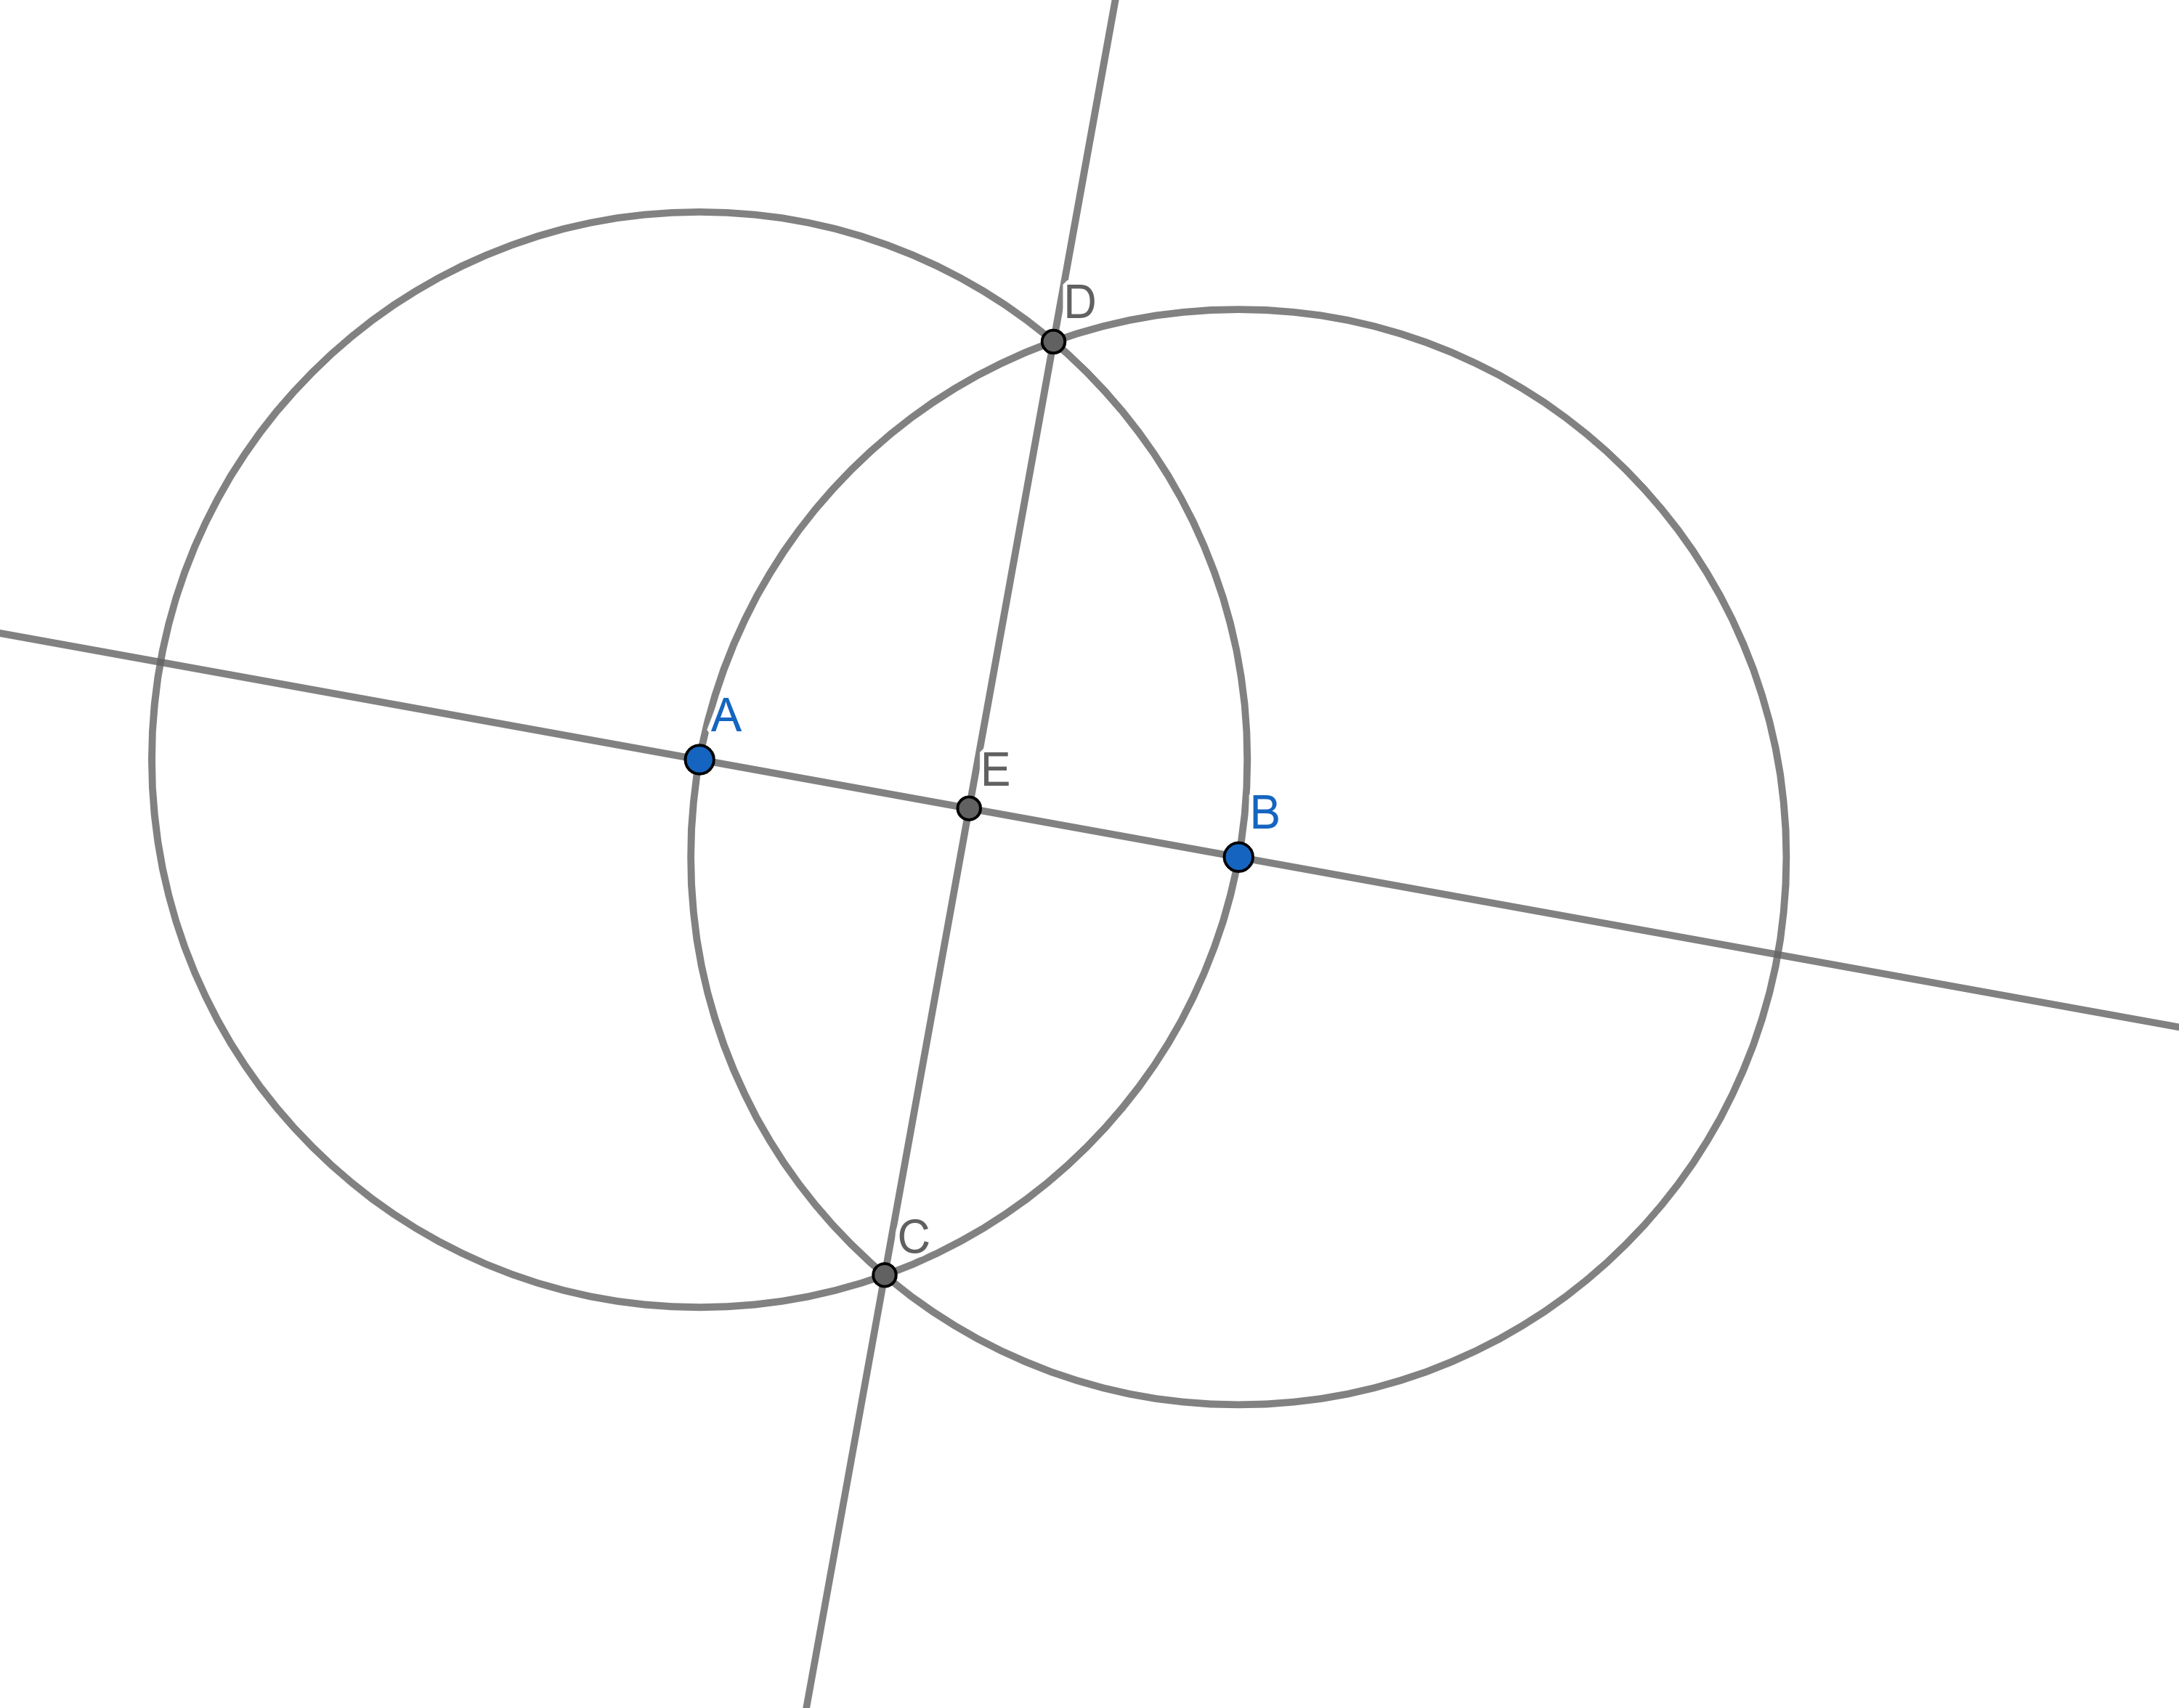
\includegraphics{geogebra-midpoint.png}}

Notice that the construction above also shows how to construct a line that is perpendicular to a given one, and how to construct an equilateral triangle.

When GeoGebra was first released the set of Geometry tools was very limited, but over time they expanded the toolkit -- after all, once you've figured out how to construct a perpendicular bisector, why not just let you click a single button to get one.  Still, some of the tools that are now available stretch the rules of Euclidean geometry.  For instance there is a proof that it's impossible to construct a regular heptagon (that would be a 7-sided polygon with all edge lengths and all angles equal), but there's a tool in GeoGebra that will let you construct a regular polygon with any number of sides that you desire.

In the lab, we're asking you to explore the notion of constructability, but many of the constructions can be accomplished with a single click if you find the right thing to click on.  Please restrict yourself to only using the tools that are ``allowed'' for each exercise.

 \clearpage
 \begin{worksheet}{15}{Geometric Constructions}{GeoGebra.png}
 \begin{enumerate}

\item Start GeoGebra, sign in, and change the mode from ``Graphing'' to ``Geometry''

\vfill

\item When you first enter the ``Geometry'' mode the tool panel will have a very limited number of options.  All but one of the things we'll need for the first task are here -- the additional tool is call ``Intersect'' and you'll need to fully expand the tool panel to find it.  Use points, lines, circles and the ability to construct points at the intersection of two curves to construct an equilateral triangle.

\vfill

\item Create a line and a point that's not on the line.  Can you use the basic tools (constructing lines and circles, finding intersections) to create a line that goes through the point, which is also perpendicular to the original line?

\vfill

\item Once you've completed the previous task, we're justified in letting you use the ``Perpendicular Line'' tool.  Using the basic tools plus ``Intersect'' and ``Perpendicular Line'' construct a square.

\vfill

\item Using the same tools, construct a right triangle where one leg is twice as long as the other.  If we say the short side is one unit long, how long is the hypotenuse of this triangle?

\vfill

\item There is a number you may have heard of called $\phi$ -- the golden proportion.  Its value is $\displaystyle \phi = \frac{1+\sqrt{5}}{2}$.
A golden rectangle is a rectangle whose side are in the golden proportion, so if you can construct a rectangle with sides $2$ and $1+\sqrt{5}$ you will have made a golden rectangle.  Referring to the previous problem, you should be able to do it!

\vfill

\item Let's finish up by exploring some properties of triangles.  Feel free to use any of the tools for these questions.
There are several ways to find a point that can be regarded as the ``center'' of a triangle.  Use Geogebra to construct all of the following:

\begin{enumerate}
	\item The line segments that go from a corner to the midpoint of the edge across from it.  There are three of these, which intersect in a point called the {\em mediant}.
	\item The line segments that are perpendicular to an edge and pass through the point across from the edge.  These intersect in a point called the {\em orthocenter}.
	\item The lines that bisect the angles at each vertex.  These intersect in a point called the {\em incenter}.
\end{enumerate}

\item Create a single triangle and construct the mediant, orthocenter and incenter.  Change the settings so that each type of ``middle'' is constructed with a different color.  Now move the corners around to see if

\begin{enumerate}
	\item it is possible to make all 3 centers coincide.
	\item it is possible to make two centers coincide while the 3rd is different.
\end{enumerate}

\end{enumerate}

 \end{worksheet}
 \clearpage


